\chapter{并发编程}

\section{多进程}

\subsection{中央处理器(CPU, Central Process Unit)}

CPU作为计算机系统的运算和控制核心,是信息处理、程序运行的最终执行单元。\\

CPU的核心部分有:

\begin{itemize}
	\item 控制单元(CU, Control Unit):控制单元是CPU的子部件,它管理着计算机中所有在这一区域执行的操作。它负责从计算机、指令和数据中获取各种输入,并告诉处理器如何处理它们。

	\item 算术逻辑单元(ALU, Arithmetic and Logic Unit):实现多组算术运算和逻辑运算的组合逻辑电路。

	\item 寄存器(register):寄存器是有限存贮容量的高速存贮部件,它们可用来暂存指令、数据和地址。
\end{itemize}

Python中可以通过multiprocessing模块获取计算机CPU的内核数量。\\

\mybox{获取CPU可用数量}

\begin{lstlisting}[language=Python]
import multiprocessing	# 导入多进程模块
# 获取CPU的可用数量
print("CPU内核数量:%d" % multiprocessing.cpu_count())
\end{lstlisting}

\vspace{0.5cm}

\subsection{进程(Process)}

Windows任务管理器提供了有关计算机性能的信息,并显示了计算机上所运行的程序和进程的详细信息。\\

进程指的是一个具有一定独立功能的程序关于某个数据集合的一次运行活动。进程是系统进行资源分配和调度运行的基本单位。进程实体中包含三个组成部分:

\begin{enumerate}
	\item 程序
	\item 数据
	\item 进程控制块(PCB, Process Control Block)
\end{enumerate}

程序(program)与进程是有区别的,程序是静态的,进程是动态的。当程序的可执行文件被装入内存后就会变成进程。进程可以认为是执行中的程序,进程需要一定资源(如CPU时间、内存、文件、I/O设备)完成任务。这些资源可以在创建的时候或者运行中分配。\\

\subsection{并发编程(Concurrent)}

并发编程是一种有效提高操作系统(服务器)性能的技术手段,现代的操作系统之中最为重要的代表就是并发性,例如现在的CPU都属于多核CPU。\\

早期的DOS操作系统有一个非常重要的特征,一旦系统沾染了病毒,那么所有的程序就无法直接执行了。因为传统的DOS系统属于单进程模型,在同一个时间段上只能运行一个程序,病毒程序运行了,其它程序自然就无法运行。\\

后来到了Windows操作系统,即便有病毒,也可以正常执行。这采用的是多进程的编程模型,同一时间段上可以同时运行多个程序。只要打开Windows的任务管理器,就可以直接清楚发现所有正在执行的并行进程。\\

在早期的硬件系统之中由于没有多核CPU的设计,利用时间片的轮转算法(Round Robin),保证在同一个时间段可以同时执行多个进行,但是在某一个时间点上只允许执行一个进程,可以实现资源的切换。

\begin{figure}[H]
	\centering
	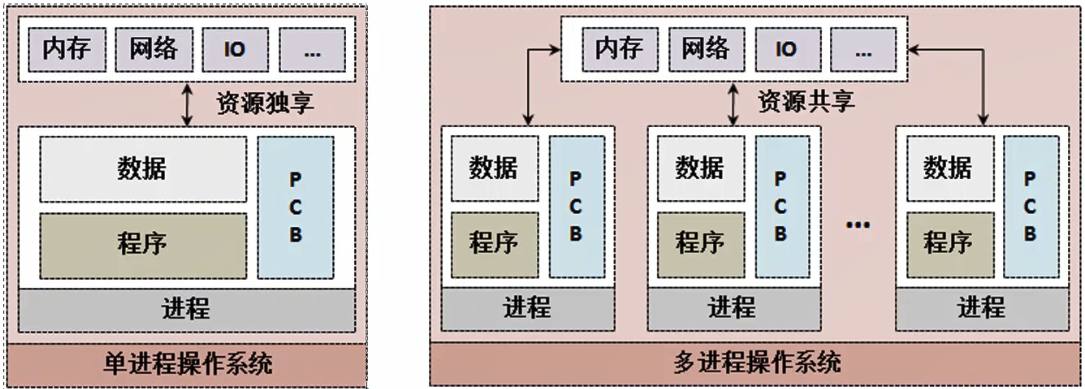
\includegraphics[scale=0.6]{img/C11/11-1/1.png}
	\caption{时间片轮转算法}
\end{figure}

服务器的硬件性能是有限的,但是对于大部分的程序来讲都属于过剩的状态。于是如果按照传统的单进程模式来运行程序,所有的硬件资源几乎都会被浪费。\\

\subsection{进程状态模型}

在两状态进程模型中,进程被分为运行态(running)和非运行态(not-running)。

\begin{figure}[H]
	\centering
	\begin{tikzpicture}[node distance=3cm,thick,auto]
		\node[state,initial] (s1) {非运行态};
		\node[state,accepting right,accepting text = {end}] (s2) [right of=s1] {运行态};

		\path[->] (s1) edge[bend left] node[above] {分配} (s2);
		\path[->] (s2) edge[bend left] node[below] {暂停} (s1);
	\end{tikzpicture}
	\caption{两态模型}
\end{figure}

并非所有进程只要是非运行态就一定处于就绪状态,有的需要阻塞等待I/O完成。因此非运行态又可分为就绪态(ready)和阻塞态(block)。\\

所有的进程从其创建到销毁都有各自的生命周期,进程要经过如下几个阶段:

\begin{enumerate}
	\item 创建状态:系统已经为其分配了PCB(可以获取进程的而信息),但是所需要执行的进程的上下文环境(context)还未分配,所以这个时候的进程还无法被调度。

	\item 就绪状态:该进程已经分配到除CPU之外的全部资源,并等待CPU调度。

	\item 执行状态:进程已获得CPU资源,开始正常提供服务。

	\item 阻塞状态:所有的进程不可能一直抢占CPU,依据资源调度的算法,每一个进程运行一段时间之后,都需要交出当前的CPU资源,给其它进程执行。

	\item 终止状态:某一个进程达到了自然终止的状态,或者进行了强制性的停止,那么进程将进入到终止状态,进程将不再被执行。
\end{enumerate}

\begin{figure}[H]
	\centering
	\begin{tikzpicture}[node distance=4.5cm,thick,auto]
		\node[state,initial] (s1) {创建};
		\node[state] (s2)[below of=s1] {就绪};
		\node[state] (s3)[right of=s2] {执行};
		\node[state] (s4)[above of=s3] {阻塞};
		\node[state,accepting below,accepting text = {end}] (s5)[right of=s3] {释放};

		\path[->] (s1) edge node[left] {许可} (s2);
		\path[->] (s2) edge[bend left] node[above] {CPU调度} (s3);
		\path[->] (s3) edge[bend left] node[below] {时间片执行完} (s2);
		\path[->] (s3) edge node[right] {产生阻塞事件} (s4);
		\path[->] (s4) edge node[left] {解除阻塞} (s2);
		\path[->] (s3) edge node {终止} (s5);
	\end{tikzpicture}
	\caption{五态模型}
\end{figure}

\newpage

\section{Process类}

\subsection{Process类}

Python中在进行多进程开发的时候可以使用multiprocessing模块进行多进程的编写,这个模块内容提供有一个Process类,利用这个类可以进行多进程的定义。所有的Python程序执行都是通过主进程开始的,所有通过Process定义的进程都属于子进程。

\begin{table}[H]
	\centering
	\setlength{\tabcolsep}{3mm}{
		\begin{tabular}{|l|l|}
			\hline
			\textbf{名称}  & \textbf{功能}                                          \\
			\hline
			pid            & 获取进程ID                                             \\
			\hline
			name           & 获取进程名称                                           \\
			\hline
			\_\_init\_\_() & 创建进程,参数target表示进程处理对象;name表示进程名称 \\
			\hline
			start(self)    & 进程启动,进入进程调度队列                             \\
			\hline
			run(self)      & 进程处理(不指定target时起效)                         \\
			\hline
		\end{tabular}
	}
	\caption{Process类}
\end{table}

所有的Python程序执行都是通过主进程开始的,所有通过Process定义的进程都属于子进程。\\

\mybox{创建多进程}

\begin{lstlisting}[language=Python]
import multiprocessing

def worker():
	"""
		进程处理函数
	"""
	print("【进程】id:%d,名称:%s" % (
		multiprocessing.current_process().pid,
		multiprocessing.current_process().name)
	)

def main():
	print("【主进程】id:%d,名称:%s" % (
		multiprocessing.current_process().pid,
		multiprocessing.current_process().name)
	)

	# 创建3个进程
	for i in range(3):
		process = multiprocessing.Process(
			target=worker, name="进程%d" % i
		)
		process.start()

if __name__ == "__main__":
	main()
\end{lstlisting}

\begin{tcolorbox}
	\mybox{运行结果}
	\begin{verbatim}
【主进程】id:4476,名称:MainProcess
【进程】id:14216,名称:进程0
【进程】id:1424,名称:进程1
【进程】id:16636,名称:进程2
\end{verbatim}
\end{tcolorbox}

\vspace{0.5cm}

\subsection{进程控制}

在多进程编程中,所有的进程都会按照既定的代码顺序执行,但是某些进程有可能需要强制执行,或者由于某些问题需要被中断,那么就可以利用Process类中提供的方法进行控制。

\begin{table}[H]
	\centering
	\setlength{\tabcolsep}{5mm}{
		\begin{tabular}{|l|l|}
			\hline
			\textbf{方法}       & \textbf{功能}    \\
			\hline
			terminate(self)     & 关闭进程         \\
			\hline
			is\_alive(self)     & 判断进程是否存活 \\
			\hline
			join(self, timeout) & 进程强制执行     \\
			\hline
		\end{tabular}
	}
	\caption{进程控制}
\end{table}

所有进程启动后,多个进程进入进程阻塞队列之中依次进行执行,那么这个时候某一个进程是不可能强占CPU的,但是通过join()可以强制执行进程。如果子进程占用的时间较长,其它的进程也需要进行等待,当子进程全部执行完毕之后就会继续执行主进程的操作。\\

所有的进程还可以进程中断处理,一般都会中断存活的进程,所以中断前需要对进程状态进行判断。但是从实际开发来讲,很少会出现强制性的霸占或者中断,否则有可能造成数据的丢失。

\newpage

\section{psutil模块}

\subsection{psutil模块}

psutil是一个进程管理的第三方模块,该模块可以跨平台(Linux、UNIX、MaxOS、Windows都支持)地进行进程管理,可以极大地简化不同系统中的进程处理操作。\\

\mybox{获取全部进程信息}

\begin{lstlisting}[language=Python]
import psutil

def main():
	# 获取全部进程
	for process in psutil.process_iter():
		print("【进程】id:%d,名称:%s,创建时间:%s" % (
			process.pid, process.name,
			process.create_time())
		)

if __name__ == "__main__":
	main()
\end{lstlisting}

除了与进程有关的操作之外,psutil模块也提供了系统硬件的内容获取。\\

\mybox{获取系统硬件信息}

\begin{lstlisting}[language=Python]
import psutil

def main():
    # CPU信息
    print("【CPU】物理数量:%d" % psutil.cpu_count(logical=False))
    print("【CPU】逻辑数量:%d" % psutil.cpu_count(logical=True))
    print("【CPU】用户用时:%f" % psutil.cpu_times().user)
    print("【CPU】系统用时:%f" % psutil.cpu_times().system)
    print("【CPU】空闲时间:%f" % psutil.cpu_times().idle)

    # 磁盘信息
    print("【磁盘】全部磁盘信息:%s" % psutil.disk_partitions())
    print("【磁盘】D盘使用率:%s" % str(psutil.disk_usage("D:")))
    print("【磁盘】IO使用率:%s" % str(psutil.disk_io_counters()))

    # 网络信息
    print("【网络】数据交换信息:%s" % str(psutil.net_io_counters()))
    print("【网络】接口信息:%s" % str(psutil.net_if_addrs()))
    print("【网络】接口状态:%s" % str(psutil.net_if_stats()))

if __name__ == "__main__":
    main()
\end{lstlisting}

\newpage

\section{Pipe进程管道}

\subsection{Pipe进程通讯管道}

进程是程序运行的基本单位,每一个程序内部都有属于自己的存储数据和程序单元,每一个进程都是完全独立的,彼此之前不能直接进行访问。但是可以通过一个特定的管道实现I/O。

\begin{figure}[H]
	\centering
	\begin{tikzpicture}
		\draw (0,0) rectangle node{工作进程} (2,1);
		\draw (4,0) rectangle node{进程管道} (6,1);
		\draw (8,0) rectangle node{工作进程} (10,1);
		\draw[->] (2,0.75) -- (3,0.75) node[above]{写} -- (4,0.75);
		\draw[<-] (2,0.25) -- (3,0.25) node[below]{读} -- (4,0.25);
		\draw[->] (6,0.75) -- (7,0.75) node[above]{写} -- (8,0.75);
		\draw[<-] (6,0.25) -- (7,0.25) node[below]{读} -- (8,0.25);
	\end{tikzpicture}
	\caption{进程间通信}
\end{figure}

\mybox{创建进程通讯管道}

\begin{lstlisting}[language=Python]
import multiprocessing

def send_data(pipe, data):
	"""
		往管道发送数据
		Args:
			pipe (Pipe): 管道
			data (str): 发送的数据
	"""
	pipe.send(data)
	print("【进程%d】发送数据:%s" % (
		multiprocessing.current_process().pid,
		data
	))

def recv_data(pipe):
	"""
		从管道接收数据
		Args:
			pipe (Pipe): 管道
	"""
	print("【进程%d】接收数据:%s" % (
		multiprocessing.current_process().pid, 
		pipe.recv()
	))

def main():
	# 管道分为发送端和接收端
	send_end, recv_end = multiprocessing.Pipe()
	# 创建两个子进程,将管道传递到对应的处理函数
	sender = multiprocessing.Process(
				target=send_data,
				args=(send_end, "Hello!")
			)
	receiver = multiprocessing.Process(
				target=recv_data,
				args=(recv_end,)
			)
	sender.start()
	receiver.start()

if __name__ == "__main__":
	main()
\end{lstlisting}

\begin{tcolorbox}
	\mybox{运行结果}
	\begin{verbatim}
【进程11664】发送数据:Hello!
【进程1032】接收数据:Hello!
\end{verbatim}
\end{tcolorbox}

\newpage

\section{进程队列}

\subsection{进程队列}

不同的进程彼此之间可以利用管道实现数据的发送和接收,但是如果发送的数据过多并且接收处理缓慢的时候,这种情况下就需要引入队列的形式来进行缓冲的操作。

\begin{figure}[H]
	\centering
	\begin{tikzpicture}
		\draw (0,0) rectangle node{生产进程} (2,1);
		\draw (4,0) rectangle node{进程队列} (6,1);
		\draw (8,0) rectangle node{消费进程} (10,1);
		\draw[->] (2,0.5) -- (3,0.5) node[above]{put} -- (4,0.5);
		\draw[->] (6,0.5) -- (7,0.5) node[above]{get} -- (8,0.5);
	\end{tikzpicture}
	\caption{生产者/消费者}
\end{figure}

multiprocessing.Queue是Python多进程编程中提供的进程队列结构,该队列采用FIFO的形式实现不同进程间的数据通讯,这样可以保证多个数据可以按序实现发送与接收处理。

\begin{table}[H]
	\centering
	\setlength{\tabcolsep}{5mm}{
		\begin{tabular}{|l|l|}
			\hline
			\textbf{方法}  & \textbf{功能}                                     \\
			\hline
			\_\_init\_\_() & 开辟队列,并设置队列保存的最大长度                \\
			\hline
			put()          & 插入数据到队列,参数timeout为阻塞超时(单位:秒) \\
			\hline
			get()          & 从队列获取数据,参数timeout为阻塞超时(单位:秒) \\
			\hline
			qsize()        & 获取队列保存数据个数                              \\
			\hline
			empty()        & 是否为空队列                                      \\
			\hline
			full()         & 是否为满队列                                      \\
			\hline
		\end{tabular}
	}
	\caption{multiprocessing.Queue类}
\end{table}

\vspace{0.5cm}

\mybox{进程队列}

\begin{lstlisting}[language=Python]
import multiprocessing
import time

def produce(queue):
	"""
		生产数据
		Args:
			queue (Queue): 进程队列
	"""
	# 生产3条数据
	for item in range(3):
		time.sleep(2)
		data = "data-%d" % item
		print("【%s】生产数据:%s" % (
			multiprocessing.current_process().name,
			data
		))
		queue.put(data)

def consume(queue):
	"""
		消费数据
		Args:
			queue (Queue): 进程队列
	"""
	while True:     # 持续消费
		print("【%s】消费数据:%s" % (
			multiprocessing.current_process().name,
			queue.get()
		))

def main():
	queue = multiprocessing.Queue()
	producer = multiprocessing.Process(
				target=produce, name="Producer",
				args=(queue,)
			)
	consumer = multiprocessing.Process(
				target=consume, name="Consumer",
				args=(queue,)
			)
	producer.start()
	consumer.start()

if __name__ == "__main__":
	main()
\end{lstlisting}

\begin{tcolorbox}
	\mybox{运行结果}
	\begin{verbatim}
【Producer】生产数据:data-0
【Consumer】消费数据:data-0
【Producer】生产数据:data-1
【Consumer】消费数据:data-1
【Producer】生产数据:data-2
【Consumer】消费数据:data-2
\end{verbatim}
\end{tcolorbox}

\newpage

\section{进程通讯}

\subsection{互斥与同步}

计算机运行过程中,大量的进程在使用有限、独占、不可抢占的资源,由于进程无限,资源有限,这种矛盾称为竞争(race)。\\

竞争条件分为两类:

\begin{enumerate}
	\item 互斥(mutex):两个或多个进程彼此之间没有内在的制约关系,但是由于要抢占使用某个临界资源(不能被多个进程同时使用的资源,如打印机)而产生制约关系。

	\item 同步(synchronization):两个或多个进程彼此之间存在内在的制约关系(前一个进程执行完,其他的进程才能执行)。
\end{enumerate}

在整个操作系统之中每一个进程都有自己独立的数据存储单元,也就是说不同进程之间无法直接实现数据共享。通过管道流可以实现进程之间的数据共享,相当于打通了不同进程之间的限制。但是不同的进程操作同一个资源就必须考虑数据同步的问题。\\

要理解同步概念,首先要清楚进程不同步所带来的问题。\\

\mybox{售票操作(Bug版本)}

\begin{lstlisting}[language=Python]
import multiprocessing
import time

def sell_ticket(dict):
	while True:     # 持续售票
		# 获取当前剩余票数
		num = dict.get("ticket")
		
		if num > 0:         # 如果还有票剩余
			time.sleep(1)   # 模拟网络延迟
			num -= 1        # 票数减1
			print("【售票员%d】售票成功,剩余票数:%d" % (
				multiprocessing.current_process().pid,
				num
			))
			dict.update({"ticket":num})     # 更新票数
		else:                				# 已经没有票了
			break

def main():
	# 创建共享数据对象
	manager = multiprocessing.Manager()
	# 创建一个可以被多个进程共享的字典对象
	ticket_dict = manager.dict(ticket=5)   # 默认有5张票

	# 创建多个售票进程
	sellers = [
		multiprocessing.Process(
			target=sell_ticket, args=(ticket_dict,)
		) 
		for _ in range(5)
	]

	for seller in sellers:
		seller.start()
	for seller in sellers:
		seller.join()   # 进程强制执行

if __name__ == "__main__":
	main()
\end{lstlisting}

\begin{tcolorbox}
	\mybox{运行结果}
	\begin{verbatim}
【售票员9732】售票成功,剩余票数:4
【售票员1640】售票成功,剩余票数:4
【售票员5976】售票成功,剩余票数:4
【售票员8048】售票成功,剩余票数:4
【售票员10516】售票成功,剩余票数:4
【售票员9732】售票成功,剩余票数:3
【售票员1640】售票成功,剩余票数:3
【售票员5976】售票成功,剩余票数:3
【售票员8048】售票成功,剩余票数:3
【售票员10516】售票成功,剩余票数:3
【售票员9732】售票成功,剩余票数:2
【售票员1640】售票成功,剩余票数:2
【售票员5976】售票成功,剩余票数:2
【售票员8048】售票成功,剩余票数:2
【售票员10516】售票成功,剩余票数:2
【售票员9732】售票成功,剩余票数:1
【售票员1640】售票成功,剩余票数:1
【售票员5976】售票成功,剩余票数:1
【售票员8048】售票成功,剩余票数:1
【售票员10516】售票成功,剩余票数:1
【售票员1640】售票成功,剩余票数:0
【售票员9732】售票成功,剩余票数:0
【售票员5976】售票成功,剩余票数:0
【售票员8048】售票成功,剩余票数:0
【售票员10516】售票成功,剩余票数:0
\end{verbatim}
\end{tcolorbox}

多个进程同时进行票数判断的时候,在没有及时修改票数的情况下,就会出现数据不同步的问题。这套操作由于没有对同步的限制,所以就造成了不同步的问题。\\

\subsection{Lock}

并发进程的执行如果要进行同步处理,那么就必须对一些核心代码进行同步。Python中提供了一个Lock同步锁机制,利用这种锁机制可以实现部分代码的同步锁定,保证每一次只允许有一个进程执行这部分的代码。

\begin{table}[H]
	\centering
	\setlength{\tabcolsep}{5mm}{
		\begin{tabular}{|l|l|}
			\hline
			\textbf{方法} & \textbf{功能}                              \\
			\hline
			acquire()     & 获取锁,如果当前没有可用锁资源,则进行等待 \\
			\hline
			release()     & 操作完毕,释放锁资源                       \\
			\hline
		\end{tabular}
	}
	\caption{Lock类}
\end{table}

\mybox{售票操作(正确版本)}

\begin{lstlisting}[language=Python]
import multiprocessing
import time

def sell_ticket(lock, dict):
	while True:     # 持续售票
		# 请求锁定,如果5秒没有锁定则放弃
		lock.acquire(timeout=5)
		
		# 获取当前剩余票数
		num = dict.get("ticket")
		
		if num > 0:         # 如果还有票剩余
			time.sleep(1)   # 模拟网络延迟
			num -= 1        # 票数减1
			print("【售票员%d】售票成功,剩余票数:%d" % (
				multiprocessing.current_process().pid,
				num
			))
			dict.update({"ticket":num})     # 更新票数
		else:                # 已经没有票了
			break
		
		lock.release()      # 释放锁

def main():
	lock = multiprocessing.Lock()   # 同步锁
	# 创建共享数据对象
	manager = multiprocessing.Manager()
	# 创建一个可以被多个进程共享的字典对象
	ticket_dict = manager.dict(ticket=5)   # 默认有5张票

	# 创建多个售票进程
	sellers = [
		multiprocessing.Process(
			target=sell_ticket, args=(lock, ticket_dict)
		) 
		for _ in range(5)
	]

	for seller in sellers:
		seller.start()
	for seller in sellers:
		seller.join()   # 进程强制执行

if __name__ == "__main__":
	main()
\end{lstlisting}

\begin{tcolorbox}
	\mybox{运行结果}
	\begin{verbatim}
【售票员14612】售票成功,剩余票数:4
【售票员15868】售票成功,剩余票数:3
【售票员13972】售票成功,剩余票数:2
【售票员10844】售票成功,剩余票数:1
【售票员2872】售票成功,剩余票数:0
\end{verbatim}
\end{tcolorbox}

一旦程序中追加了同步锁,那么程序的部分代码就只能以单进程执行了,这样势必会造成程序的执行性能下降,只有在考虑数据操作安全的情况下才会使用锁机制。\\

\subsection{Semaphore}

Semaphore(信号量)是一种有限资源的进程同步管理机制。例如银行的业务办理,所有客户都会拿到一个号码,而后号码会被业务窗口叫号,被叫号的办理者就可以办理业务。\\

Semaphore类本质上是一种带有计数功能的进程同步机制,acquire()减少计数,release()增加计数。当可用信号量的计数为0时,后续进程将被阻塞。\\

Lock一般是针对于一个资源同步的,而Semaphore是针对有限资源的并行访问。\\

\mybox{信号量同步处理}

\begin{lstlisting}[language=Python]
import multiprocessing
import time

def work(sema):
	if sema.acquire():      # 获取信号量
		print("【进程%d】开始办理业务" % 
			multiprocessing.current_process().pid)
		time.sleep(2)       # 模拟办理业务
		print("【进程%d】结束办理业务" % 
			multiprocessing.current_process().pid)
		sema.release()      # 释放资源

def main():
	# 允许3个进程并发执行
	sema = multiprocessing.Semaphore(3)
	workers = [
		multiprocessing.Process(target=work, args=(sema,))
		for _ in range(10)
	]

	for worker in workers:
		worker.start()
	for worker in workers:
		worker.join()

if __name__ == "__main__":
	main()
\end{lstlisting}

\begin{tcolorbox}
	\mybox{运行结果}
	\begin{verbatim}
【进程7880】开始办理业务
【进程3032】开始办理业务
【进程5412】开始办理业务
【进程7880】结束办理业务
【进程2876】开始办理业务
【进程3032】结束办理业务
【进程14076】开始办理业务
【进程5412】结束办理业务
【进程8816】开始办理业务
【进程2876】结束办理业务
【进程14076】结束办理业务
【进程7900】开始办理业务 
【进程7860】开始办理业务 
【进程8816】结束办理业务 
【进程16252】开始办理业务
【进程7860】结束办理业务
【进程7900】结束办理业务
【进程972】开始办理业务
【进程16252】结束办理业务
【进程972】结束办理业务
\end{verbatim}
\end{tcolorbox}

\newpage